\chapter{Password-less Authentication and Identification}
\label{chp::deeid}

This chapter designs and implements a passwordless system---\deeid---for identification to mitigate impersonation attacks. \deeid is a blockchain-based system that enables passwordless authentication and identification by extending the Fiat--Shamir protocol to support multiple identity issuers. Blockchain is used as a decentralised public-key infrastructure, providing identity verification without relying on passwords or centralised authorities while maintaining compatibility with existing web technologies.

The source code for the implementation can be found at \url{https://github.com/deeid}.

\section{Introduction}
\label{sec::chp6::introduction}
%\begin{figure}[ht]
%\centering
%\noteBox{Identification}{
%Here we make a distinction between \textit{Identification} and \textit{authentication} as per the Fiat--Shamir~\cite{fiat_how_1986} definitions. Consider a universe of users $U = \{u_1, u_2, ..., u_n\}$ and a proof function $P(x,y,c)$ where $x$ proves to verifier $c$ that they are user $y$, returning true if successful and false otherwise. Formally, $P: U \times U \times U \rightarrow \{\text{true}, \text{false}\}$. Authentication requires that for any user $A$ and verifier $B$, $A$ can prove their identity $(P(A,A,B) = \text{true})$ while no other user $X$ can successfully claim to be $A$ $(\forall X \neq A: P(X,A,B) = \text{false})$. Identification strengthens this by adding the constraint that even the verifier $B$ cannot replay $A$'s proof to impersonate them $(\forall X \neq A: \forall Y: P(B,A,Y) = \text{false})$. This hierarchy establishes that: 
%$$\text{Identification} \implies \text{Authentication}$$
%$$\text{Authentication} \not\implies \text{Identification}$$
%capturing the distinction that identification prevents replay attacks while authentication only prevents initial impersonation.
%}
%\end{figure}

Many organisations and digital identity systems rely on a fundamentally flawed premise for identification: using shared secrets for verification. Every time you enter a password, provide your date of birth, or answer security questions, you share reusable information that can be stolen, intercepted, or replayed by attackers. Most often, these supposed \textit{secrets} are publicly available information, such as your date of birth. This approach creates systemic vulnerabilities throughout the digital ecosystem that lead to identity theft and impersonation attacks.

Well-resourced and motivated attackers exploit these shared secret systems: in one incident, an attacker used deepfake technology to impersonate a company executive, successfully convincing an employee to transfer US\$25~million~\cite{milmo_uk_2024}. In another case, an attacker compromised the SEC's Twitter/X account using a SIM-swapping attack facilitated by a fake ID and impersonation~\cite{kan_hijack_2024}. These cases demonstrate that we should seldom rely on readily available information for authentication and identification.

Our idea is to replace all shared-secret systems with interactive challenge-response protocols in which identity verification reveals nothing reusable, enabled by dynamic trust networks that allow any organisation to issue identities that work across national borders.

We call this system \deeid and this is how it works: It extends the Fiat-Shamir identification protocol to work with multiple identity issuers, using the blockchain as a decentralised public key infrastructure. When you need to prove your identity, the system generates a cryptographic challenge to which you respond using private keys stored on your mobile device. This response proves that you possess the correct credentials without revealing any secret information that could be reused. Identity issuers (banks, governments, universities) can create and verify these credentials using a shared blockchain ledger, but no single authority controls the system---hence the dynamic trust network.

The novelty of \deeid is in adapting the classical Fiat-Shamir scheme, originally designed for single-issuer scenarios, to work seamlessly with multiple independent identity providers. Users can obtain \textit{many} digital identities on the blockchain provided by different organisations. Verifiers can check these credentials through interactive proofs rather than through shared-secret verification. Having many sources of identities is positive as it mitigates a single point of failure and verifiers can use this to verify consistency across identities.

Unlike password systems which rely on shared secrets, \deeid reveals nothing reusable during verification. Unlike federated identity systems which create vendor lock-in, \deeid enables any organisation to issue credentials that work with any other organisation's verification systems. Unlike traditional PKI systems which require centralised certificate authorities, deeID uses blockchain to create a decentralised trust infrastructure. WebAuthn is primarily designed for authentication, \deeid is designed for identification. \deeid predates Passkeys (which is an implementation of WebAuthn and the relevant standards).

The benefits of this approach are numerous. It eliminates the security weakness of shared secrets—there is nothing for attackers to steal or replay; it preserves privacy through the zero-knowledge proof of identity. It enables interoperability where identities issued by one organisation can be verified by any other organisation in the network. Finally, it creates a foundation for dynamic trust networks where identity verification can adapt to real-world relationships rather than being constrained by centralised authorities.

%This chapter represents not only a step in our journey of protecting user secrets but also a vision and a fundamental shift in how we think about identification and authentication---moving from what you know (passwords, personal information) to stronger forms of identification and authentication. WebAuthn and passkeys have made enormous strides since 2022 in moving beyond passwords. While this chapter addresses authentication, it primarily focuses on the challenges of identification, as exemplified by the real-world examples in the previous paragraph.

%Decentralisation is motivated and achieved using Blockchain. Blockchain has proven to have numerous important applications beyond its initially conceived purpose of digital cash (Bitcoin~\cite{nakamoto_bitcoin:_2009} since 2009). Its use as a public-key infrastructure (PKI) and in identity management represents two significant examples with considerable implications for web applications. Namecoin~\cite{noauthor_namecoin_nodate}, Blockstack~\cite{noauthor_blockstack_nodate}, and Certcoin~\cite{fromknecht_certcoin_2014} exemplify organisations attempting to recreate DNS, identity, and certification services using Blockchain. Additional implementations utilising Blockchain as a PKI include applications for IoT devices~\cite{pinto_blockchain-based_2020} and identity management~\cite{boontaetae_rdi:_2018}.

%\textbf{Threat\;Scenario.}\; Modern attackers exploit identity weaknesses not only through sophisticated social engineering campaigns but also through insider threats and compromised services. While traditional security models assume services can be trusted, we must consider that the very systems we authenticate with may be adversarial. Insiders with privileged access can bypass security controls, exfiltrate identity data, or manipulate authentication processes. Service providers themselves may be compromised, coerced, or simply negligent in protecting identity information. By combining publicly available information with AI-generated content and insider knowledge, attackers can build highly convincing attacks that exploit both technical vulnerabilities and human trust relationships. This interconnected nature of identity systems, coupled with the necessity to treat authentication services as potentially hostile actors, means that a compromise in one area can cascade into unauthorised access across multiple domains.

%Identity verification relies on layers of proof, with each document typically deriving its authority from another. People accumulate multiple forms of identification throughout their lives, from birth certificates to passports and driver's licences. Organisations often require several of these documents because forging multiple forms of identification costs more time and resources than most criminals can afford to spend. This layered approach builds trust through accumulated proof: as people conduct more transactions and interact with more institutions, they establish a deeper foundation of verified identity. However, many online services have abandoned this protective layering in favour of simplified verification. They often require only basic personal details, such as names, addresses, and birthdates, to open credit cards or insurance policies. Even phone-based authentication typically demands just these surface-level facts, making digital identity theft significantly easier than forging traditional documents. This weakness in online verification undermines the security that traditional layered identification systems provide.

%This concept of \textit{identity credit} remains vulnerable to criminal exploitation through \textit{synthetic identity fraud}~\cite{noauthor_combating_nodate}. In this scheme, criminals fabricate fictional identities and establish legitimate financial and credit histories for them. This manufactured credibility makes the identity appear genuine to challengers. However, it merely serves as a stepping stone for criminals to gain access to larger credit facilities and finances. This vulnerability is perpetuated, in part, by the absence of a common, trusted service that all organisations could use for identity verification.

%The benefits of the proposed system are numerous. Firstly, the most obvious application is the replacement of username and password combinations for authentication. With a secure, up-to-date, and decentralised key-store, it presents a practical alternative, particularly considering potential cost savings regarding lost passwords~\cite{wolfond_blockchain_2017}. Secondly, it provides a straightforward method to prove one's identity online through identity providers (e.g., your bank can serve as a trusted identity provider). Thirdly, it can help reduce phone scams, identity fraud, and related crimes by ensuring that access relies less on common personal information and more on a combination of ``what we possess'' (a mobile phone with strong private keys) or ``what we know'' combined with ``what we have'' (fingerprint access to our mobile phones). Finally, it introduces flexibility and consistent standards to organisations, countries, and continents where gaps in standards and trust exist.

%\section{Selective Disclosure Theory}
\label{sec::chp6::selective-disc-theory}

\begin{figure}[h!]
    \centering
\begin{tikzpicture}[font=\small, node distance=2.5cm, >=latex, 
  every node/.style={draw, rectangle, minimum width=1.2cm, minimum height=0.8cm, align=center},
  level/.style={sibling distance=2cm, level distance=1.5cm}]

  %%% Leaves (Merkle tree leaves)
  \node (L1) at (0,0) {$L_1 = H(s_1^\text{(salt)} \| a_1)$};
  \node (L2) at (4,0) {$L_2 = H(s_2^\text{(salt)} \| a_2)$};
  \node (L3) at (8,0) {$L_3 = H(s_3^\text{(salt)} \| a_3)$};
  \node (L4) at (12,0) {$L_4 = H(s_4^\text{(salt)} \| a_4)$};
  
  %%% Internal nodes (hashes of leaves)
  \node[circle] (H12) at (2,2) {$H_{1,2}$};
  \node[circle] (H34) at (10,2) {$H_{3,4}$};
  
  %%% Root node
  \node[circle] (R) at (6,4) {$R$};

  %%% Draw edges
  \draw[->] (L1) -- (H12);
  \draw[->] (L2) -- (H12);
  \draw[->] (L3) -- (H34);
  \draw[->] (L4) -- (H34);
  \draw[->] (H12) -- (R);
  \draw[->] (H34) -- (R);

  %%% Label internal nodes with how they're derived (optional)
  \node[above=0.1cm of H12, draw=none] {\small $H_{1,2} = H(L_1 \| L_2)$};
  \node[above=0.1cm of H34, draw=none] {\small $H_{3,4} = H(L_3 \| L_4)$};
  \node[above=0.1cm of R, draw=none] {\small $R = H(H_{1,2} \| H_{3,4})$};

  %%% Highlight the path for L2 (selective disclosure)
  \draw[very thick, color=blue] (L2) -- (H12);
  \draw[very thick, color=blue] (H12) -- (R);

  %%% Optionally, add a legend or annotation
  % Mark the "disclosed path" in blue
  \node[draw=none, text width=4cm, align=left, anchor=west] at (3,-1.3)
  {\textcolor{blue}{\textbf{Disclosed Path}}: \\
   $(L_2 \rightarrow H_{1,2} \rightarrow R)$};

\end{tikzpicture}
    \caption{Selective disclosure in a Merkle tree. The diagram illustrates a four-attribute identity structure with leaf nodes $L_j = H(s_j^{\text{(salt)}} \| a_j)$. The blue path highlights the selective disclosure of attribute $a_2$, where only $L_2$ and the auxiliary path information $(L_2, H_{1,2}, R)$ are revealed, enabling verification against the root $R$ without exposing the undisclosed attributes $a_1$, $a_3$, and $a_4$. This demonstrates how Merkle proofs facilitate attribute verification while preserving privacy.}    

    \label{fig::chp6::selective-disclosure}
\end{figure}

\subsection{Overview}

Treating services as adversarial dictates that we should reveal as little information as possible. While Fiat--Shamir zero-knowledge cryptosystems ensure that secrets themselves are not disclosed, they still require revealing various attributes of our identity. However, in real-world scenarios, a prover often needs to disclose only some attributes rather than all. For example, someone proving that they are German does not need to reveal other identity attributes. This is where \textit{Selective Disclosure} of identity attributes becomes crucial. We combine the Fiat--Shamir~\cite{fiat_how_1987} cryptosystem with a Merkle~tree~\cite{merkle1987digital} construction to selectively reveal certain attributes while keeping others hidden.

The proposed approach combines the Fiat--Shamir zero-knowledge cryptosystem with a Merkle tree construction to achieve selective disclosure of identity attributes. Specifically, each attribute $a_i \in \mathcal{A}$ is hashed with a random salt $s_i^{\text{(salt)}}$ to create leaf nodes $L_i = H(s_i^{\text{(salt)}} \,\|\, a_i)$ in a Merkle tree with root $R$. During the disclosure protocol, the prover reveals only the selected attributes along with their corresponding salts and Merkle inclusion proofs $\pi_j$, while executing a Fiat--Shamir proof using secret values $s_j$ tied to these attributes. This novel combination ensures that undisclosed attributes remain hidden due to the Merkle tree's structural properties, while the cryptographic binding between the attributes and the identity credentials is maintained through the Fiat--Shamir protocol, effectively addressing the limitation of traditional zero-knowledge systems that require revealing all identity attributes.

\subsection{Preliminaries and Setup Phase}

Our selective disclosure protocol operates on a set of identity attributes $\mathcal{A} = \{a_1, a_2, ..., a_m\}$, where each $a_i$ represents a statement about identity (e.g., ``\textit{over 18}'', ``\textit{British Citizen}''). The cryptographic foundation rests on three key components: a secure cryptographic hash function $H: \{0,1\}^* \rightarrow \{0,1\}^l$, a Merkle tree construction $\mathcal{MT}$ capable of generating and verifying inclusion proofs, and an RSA modulus $n = pq$ where $p$ and $q$ are large primes.

For each attribute $a_i \in \mathcal{A}$, we generate a unique random salt and then compute a salted hash commitment:
$$L_i = H(s_i^{\text{(salt)}} \,\|\, a_i)$$

Next, we build the Merkle tree from the leaves $L_i$. The Merkle root $R$ becomes our identity string (which is represented as $I$ in the Fiat--Shamir protocol.)

\paragraph{Key\;Generation.}\;We follow the Fiat--Shamir protocol and have a trusted identity issuer create $v_j = f(R, j) \mod n$.

\paragraph{Selective Disclosure Protocol.} To prove an attribute $a_i$:
\begin{itemize}
    \item Disclose $a_i$
    \item Provide the Merkle path for $L_i$
    \item Perform Fiat--Shamir interaction to prove knowledge of $s_j$, using $R$ as the public identity.
\end{itemize}
%During the setup phase, we commit to each attribute through a carefully constructed salting mechanism. For each attribute $a_j \in \mathcal{A}$, we generate a unique random salt $s_j^{\text{(salt)}} \stackrel{R}{\leftarrow} \{0,1\}^k$ and compute a salted hash commitment:


These leaf nodes $\{L_1, \ldots, L_m\}$ are then organised into a Merkle tree $\mathcal{MT}$, culminating in a root $R$ that serves as a succinct cryptographic commitment to the entire attribute set. This elegant construction achieves two essential objectives: it enables efficient verification of attribute membership during disclosure, while the tree's structural properties ensure undisclosed attributes remain hidden from verifiers. The salting mechanism further strengthens privacy by ensuring that even identical attributes yield distinct leaf hashes, effectively thwarting dictionary attacks and enhancing the overall security of our selective disclosure protocol.


%\subsection{Selective Disclosure Protocol}
%
%Suppose the prover wants to \emph{selectively} disclose a subset of
%their attributes, indexed by $\mathcal{D} \subset \{1,\ldots,m\}$. In
%other words, the prover wants to prove possession of $(a_j)_{j\in \mathcal{D}}$
%and also execute a Fiat-Shamir-like proof tied to those attributes
%\emph{without} revealing the undisclosed attributes $\{a_j: j\notin\mathcal{D}\}$.
%
%\subsubsection*{Prover (Commitment):}
%
%\begin{enumerate}
%    \item Choose a random $r \stackrel{R}{\leftarrow} \mathbb{Z}_n^*$.
%    \item Compute $x = r^2 \bmod n$.
%    \item For each disclosed attribute index $j \in \mathcal{D}$, retrieve the 
%    corresponding Merkle-leaf hash $L_j$ and generate a Merkle inclusion 
%    proof $\pi_j = \text{MerkleProof}\bigl(j, L_j, \mathcal{MT}\bigr)$ 
%    that convinces a verifier that $L_j$ is indeed in the Merkle tree 
%    with root $R$.
%    \item Send $(\,x,\; \{\,(\,a_j,\;s_j^\text{(salt)},\;\pi_j\,)\}_{j \in \mathcal{D}}\,)$ 
%    to the verifier. Here, $a_j$ and $s_j^\text{(salt)}$ allow the verifier 
%    to recompute $L_j = H(s_j^\text{(salt)}\|\;a_j)$ and check it against 
%    the Merkle proof $\pi_j$ and root $R$.
%\end{enumerate}
%
%\subsubsection*{Verifier (Challenge):}
%
%\begin{enumerate}
%    \item The verifier checks each provided Merkle proof $\pi_j$ for 
%    correctness by ensuring that $L_j$ indeed corresponds to the path 
%    that leads to root $R$.
%    \item The verifier also checks that $L_j = H\bigl(s_j^\text{(salt)}\|\;a_j\bigr)$ 
%    for each disclosed attribute $j \in \mathcal{D}$.
%    \item If these checks succeed, the verifier issues a random challenge 
%    \[
%        e = \bigl(e_1,e_2,\dots,e_m\bigr),
%    \]
%    where each $e_j$ is typically 1 bit (or a small number of bits), 
%    and only $e_j$ for $j \in \mathcal{D}$ are relevant (the others 
%    can be set to 0, or the subset structure can be indicated in some 
%    canonical way).
%\end{enumerate}
%
%\subsubsection*{Prover (Response):}
%
%\begin{enumerate}
%    \item Compute the response
%    \[
%       y \;=\; r \;\prod_{j \in \mathcal{D}}\, s_j^{\,e_j}
%       \;\bmod n.
%    \]
%    \item Send $y$ to the verifier.
%\end{enumerate}
%
%\subsubsection*{Verifier (Final Check):}
%
%The verifier checks the core Fiat-Shamir equation:
%
%\[
%    x \;\stackrel{?}{=}\; 
%    \Bigl(y^2 \;\prod_{j \in \mathcal{D}}\; v_j^{\,e_j}\Bigr)
%    \bmod n.
%\]
%
%If this congruence holds, the verifier accepts; otherwise the verifier 
%rejects.
%
%\subsection{Security Analysis}
%
%\subsubsection{Zero-Knowledge}
%
%\begin{enumerate}
%    \item \textbf{Attribute Hiding via Merkle Tree.} 
%    The attributes that are not disclosed do not appear in any revealed 
%    path of the Merkle tree, hence they remain hidden.
%    \item \textbf{Fiat-Shamir Zero-Knowledge.}
%    The standard Fiat-Shamir protocol is zero-knowledge in the random 
%    oracle model. The responses $(r, y)$ and challenge $e$ reveal no 
%    additional information about undisclosed $s_j$ values.
%    \item \textbf{Salts Prevent Dictionary Attacks.}
%    Using per-attribute salts $s_j^\text{(salt)}$ when computing 
%    $L_j = H\bigl(s_j^\text{(salt)}\|\,a_j\bigr)$ ensures that an 
%    attacker cannot simply guess attributes and verify them offline 
%    (i.e., a brute-force or dictionary attack).
%\end{enumerate}
%
%\subsubsection{Soundness}
%
%\begin{enumerate}
%    \item \textbf{Merkle Tree Binding.} 
%    Because $R$ is the root of the Merkle tree, any attempt to forge 
%    attributes would cause the Merkle proof to fail or produce an 
%    incorrect leaf.
%    \item \textbf{Fiat-Shamir Soundness.} 
%    The classical Fiat-Shamir soundness argument (in the random oracle 
%    model or in a challenge-response setting) prevents impersonation: 
%    forging a correct response for non-owned $s_j$ with high probability 
%    is infeasible.
%    \item \textbf{Binding Attributes to the Root.} 
%    The root $R$ binds the set of attributes to the user's identity 
%    credentials. Any modifications to a claimed attribute would require 
%    recomputing the root, thus invalidating the public key.
%\end{enumerate}
%
%\subsubsection{Completeness}
%
%For an honest prover who possesses all secret values $s_j$ and the random commitment $r$, the verification always succeeds. We can demonstrate this by examining the verification equation. The prover computes response $y = r\prod_{j \in \mathcal{D}} s_j^{e_j} \bmod n$, which gives us:
%
%$$
%y^2 = r^2\prod_{j \in \mathcal{D}} s_j^{2e_j} \bmod n
%$$
%
%Since each $v_j = s_j^{-2} \bmod n$, we have:
%
%$$
%\prod_{j \in \mathcal{D}} v_j^{e_j} = \prod_{j \in \mathcal{D}} (s_j^{-2})^{e_j} = \prod_{j \in \mathcal{D}} s_j^{-2e_j} \bmod n
%$$
%
%Combining these expressions in the verification equation:
%
%$$
%y^2 \prod_{j \in \mathcal{D}} v_j^{e_j} = \left(r^2 \prod_{j \in \mathcal{D}} s_j^{2e_j}\right) \left(\prod_{j \in \mathcal{D}} s_j^{-2e_j}\right) = r^2 \bmod n
%$$
%
%The verifier's check $x \stackrel{?}{=} y^2 \prod_{j \in \mathcal{D}} v_j^{e_j}$ succeeds precisely because $x = r^2 \bmod n$, thus confirming the protocol's completeness property.

\section{Threat Scenario}
\label{sec::chp6::threat_scenario}

Attackers exploit identity weaknesses not only through sophisticated social engineering campaigns but also through insider threats and compromised services. While traditional security models assume services can be trusted, we must consider that the very systems we authenticate with may be adversarial. Insiders with privileged access can bypass security controls, exfiltrate identity data, or manipulate authentication processes. Service providers themselves may be compromised, coerced, or simply negligent in protecting identity information.

By combining publicly available information with AI-generated content and insider knowledge, attackers can build highly convincing attacks that exploit both technical vulnerabilities and human trust relationships. This interconnected nature of identity systems, coupled with the necessity to treat authentication services as potentially hostile actors, means that a compromise in one area can cascade into unauthorised access across multiple domains.

\section{Design}
\label{sec::chp6::design}

Our aim is to create an identity system that: (1) preserves privacy through zero-knowledge proofs, (2) supports multiple identity issuers in a decentralised way, (3) maintains compatibility with existing infrastructure, and (4) provides stronger security guarantees than current systems. While WebAuthn solves the authentication problem well, it does not address the broader identity management and verification challenges that \deeid attempts to solve. The novel contribution would be in creating a comprehensive identity framework that extends beyond simple authentication to handle complex real-world identity verification scenarios.

The \deeid is designed to function with mobile devices. Identity holders require a mobile phone capable of securely storing private keys using device-level encryption or secure enclave technology. The deeID application manages these keys, performs cryptographic operations, scans QR codes, and maintains WebSocket communication with verifiers. On the service side, integration is lightweight: Web applications employ JavaScript libraries to generate QR codes that contain session identifiers and challenges. When a user scans such a code, their mobile device initiates a WebSocket session with the service and executes the interactive authentication protocol. Importantly, no browser extensions or modifications are required. Browsers are used only to display QR codes and to confirm completed authentication, while all cryptographic operations remain confined to the user's device.

The \deeid system involves four primary actors:

\begin{itemize}
    \item Identity Holders are individuals who own and control their digital identities. Each identity holder possesses a unique blockchain-based smart contract that serves as their identity anchor, along with private keys stored on their mobile device for cryptographic operations.
    
    \item Identity Issuers are organisations (banks, universities, governments, employers) that can create and issue credentials to identity holders. Each issuer maintains their own smart contract containing cryptographic parameters used in the Fiat-Shamir protocol.
    
    \item Verifiers are services or organisations that need to authenticate identity holders. They may maintain lists of trusted issuers and can verify credentials through interactive cryptographic challenges without accessing any shared secrets.
    
    \item The Blockchain Network serves as the decentralised public key infrastructure, storing smart contracts, public keys, and issuer parameters while ensuring that no single authority controls the system.
\end{itemize}

%%%%


%%%%

\paragraph*{Other requirements:} \deeid is designed with the following requirements:

\textbf{Compatibility.} Compatible with existing browsers and existing technology that use the email/password combination for authentication. The user must not download new browsers. Developers should be able to use existing JavaScript or Python web stacks to implement \deeid\ as an authentication scheme.

\textbf{Key Store Management.} Shared and equal access to public keys that link users to their identities, ensuring transparency and verifiability within the system. This assumes that a user can possess multiple keys (e.g., for different devices and keys for encryption), allowing flexibility and enhanced security across various use cases.

\textbf{Dynamic Identity.} Ability for anyone to issue identities to individuals. Utilise and implement the Fiat--Shamir scheme for multiple identity issuers.

\textbf{Privacy by Design.} Cannot record any personal details on the public chain.

\textbf{Unlinkable Authentication} Colluding actors cannot determine if our anonymous identity is the same across their servers and systems.

\noteBoxNormal{Requirements}{%
    Steps required before an entity can issue an identity: \\
    Person \textbf{A}: The individual wishing to receive a new identity from another person or organisation.
    
    Person \textbf{B}: Identity issuer.
    
    \begin{enumerate}
        \item \textbf{A}: Must create a \deeid\ representation on the blockchain, e.g. on Ethereum, create a unique contract as per the common standards.
        \item \textbf{B}: Must also create a \deeid\ representation on the network.
        \item \textbf{B}: Create a random modulus which is a product of two large prime numbers, $n = pq$, and n should be at least 512~bits.
        \item \textbf{B}: Store $n$ on the network. In our implementation it is stored in a data structure on the \deeid\ contract.
    \end{enumerate}
}
%%%%%%%%%%%%%%%%%%%%%%%%%%%%%%%%%%%%%%%%%%%%%%%%%%%%%%%%%%%%%%%%%%%%%%%%%%%%%%%%%%%%%%%%%%%
\section{Implementation}
\label{sec::chp6::implementation}

\subsection{Overview}
\begin{figure}[t]
    \center{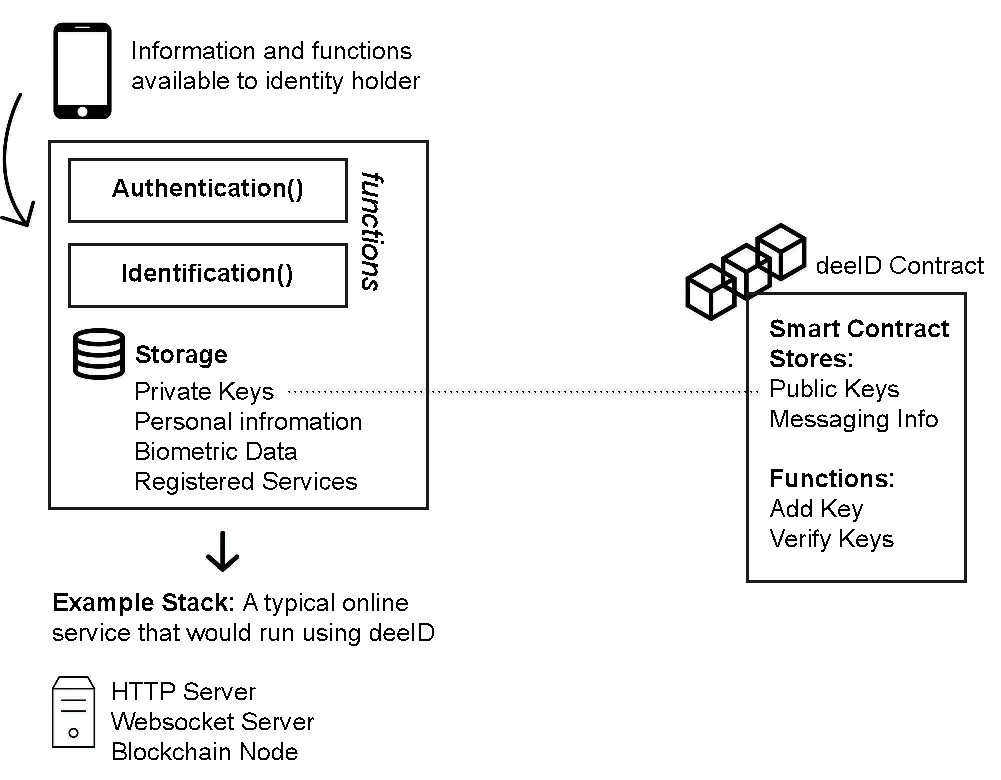
\includegraphics[scale=0.5]
    {figs/deeid/deeID_diagram.pdf}}
    \caption{\label{fig:deeIDArchitecture} \deeid architecture overview. \srcOwnFig}
\end{figure}

The proposed system, \deeid, is a combination of technologies that enables a dynamic and decentralised identity system with functions compatible with existing services.
Although the proposed system can be built on various devices, even a unique independent device solely for this application, we have assumed the implementation on a typical mobile device running Android or iOS.
\deeid uses the Fiat--Shamir identification cryptosystem with a blockchain~that~acts~as~a~PKI.

Figure \ref{fig:deeIDArchitecture} provides an overview of the system. The core components are:
\begin{itemize}
    \item \textbf{Distributed\;Ledger:}\;Our implementation uses Ethereum and we have developed several smart-contracts that act as portals and identity managers.
    \item \textbf{Mobile\;Phone:}\;A device such as a mobile phone that can store private keys and interact with services and servers over the Internet (in part to ensure compatibility with existing web applications). We built a mobile phone application that allows the user to authenticate and identify (Fiat--Shamir scheme) themselves. The application uses QR codes to interact with web applications and then talk to servers (using WebSocket connection) to carry out the necessary functions (e.g. interactive Fiat--Shamir scheme).
    \item \textbf{Libraries:}\;Required libraries that developers can install so that their users can use \deeid to authenticate themselves on the developer's application.
\end{itemize}

\noteBox{Analogy}{
To effectively showcase the potential of \deeid, one could employ the analogy of an identity card. Figure~\ref{fig:idcard} illustrates this analogy, highlighting the three primary elements of an identity card:
\vspace{0.25cm}

\textbf{Photograph for verification:} We typically use the photograph of the individual on the identity card to identify the user. That is, the assumed valid ID card belongs to the individual trying to prove their identity to the challenger. In \deeid, this is done by the ownership of a private key associated with an identity. Via the Fiat--Shamir scheme, one would be able to prove their ownership of the private-key~and,~therefore,~identity.
\vspace{0.25cm}

\textbf{Human and machine readable strings:} We require a unique string that would uniquely identify the card. This string can also be used for record keeping with respect to the identity holder. Along with this unique string, we also have the full name of the user. Although it is typically not unique. However, it is what we use to identify with one another at the human level. In \deeid, the smart contract on the network with its unique address represents the unique~machine-readable~identity.
\vspace{0.25cm}

\textbf{Identity issuer's integrity:} The integrity of the identity card comes through trusting the physical card itself and its physical properties. This trust also assumes that the verifier trusts the organisation that has issued the card. We find organisations that require different proofs of identity, e.g. passport and driving license in the UK. Therefore, we are concerned with different issuers and their reputation. Reputation in itself would require a full research experiment; in the current state of \deeid we have used a simple link on the identity issuer's smart contract, which links to their web address if they have one proving that the owner has access to both.
}

\begin{figure}[h]
    \center{
    \textbf{Relating \deeid to an Identity Card}\par\medskip
    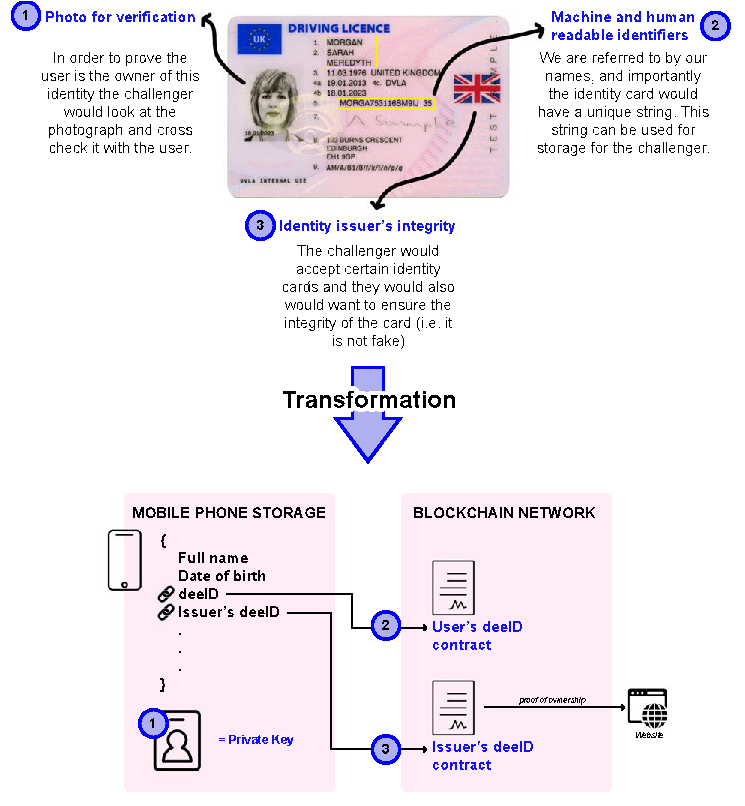
\includegraphics[scale=0.65]
    {figs/deeid/id_card.pdf}}
    \caption{At the top we have the main components of an identity card and at the bottom we have the equivalent functions in \deeid. \srcOwnFig}
    \label{fig:idcard}
\end{figure}


\subsection{Decentralised Public Key Infrastructure}
\label{sec::chp6::dpki}

A fundamental challenge in extending a scheme, such as the Fiat--Shamir scheme, to multiple identity issuers is a trustworthy and robust public-key management infrastructure. We leverage the decentralised public key infrastructure (DPKI) to enable \deeid to handle multiple identity issuers at the same time. Numerous studies have contributed to decentralised PKI (DPKI)~\cite{kubilay_certledger:_2019, dykcik_blockpki:_2018, yakubov_blockpgp:_2018, patsonakis_practicality_2019} and here we represent a simple solution built on Ethereum for \deeid. With this approach, the user can associate other public-keys to their identity, e.g. RSA keys for encryption and public-keys used on other devices that links back to the identity.

Our DPKI implementation diverges from traditional certificate-based systems by anchoring key authenticity directly to verifiable identities. This represents a paradigm shift: instead of relying on certificate chains, we establish trust through the identity verification process itself. While existing DPKI solutions~\cite{kubilay_certledger:_2019, dykcik_blockpki:_2018, yakubov_blockpgp:_2018, patsonakis_practicality_2019} focus on certificate management, our approach integrates identity verification with key management.

We assume that the user has ownership control of their \deeid smart contract, and thus any changes within the contract are not malicious. Furthermore, the integrity of the public keys falls under the actual \deeid, and individual public keys are not issued certificates as such. So, if a verifier has no knowledge of the user's \deeid, then they must first identify the \deeid user (through the Fiat--Shamir scheme).

Adding new public keys to the smart contract \deeid is a simple process of invoking the \texttt{addKey()} function with the following arguments: \texttt{title}, \texttt{key} and \texttt{comment}. The criterion for adding the key is that the user must be the owner of \deeid---which in our implementation has been cross-checking the sender's address with the address of the owner (stored on the smart contract). A real-world application could use any of the keys stored on the \deeid to verify the integrity of the sender. Lastly, verifying a specific key would involve querying the blockchain with respect to the public key and \deeid, in our implementation we had a function \texttt{getKey()}, which would return all the details related to that key.

Other blockchain-based PKIs are more traditional in that they use certifications, e.g. CertLedger~\cite{kubilay_certledger:_2019}  and CertCoin~\cite{fromknecht_decentralized_2014}. In \deeid authenticity and security come from the identification of the \deeid itself, which can depend on the identity issuer and the verifier's willingness to trust the issuer or not. Although in the current implementation of \deeid this verifier and issuer trust is not quantified, we envision that one would be able to add a quantifiable reputation layer.

\subsection{Authentication}
The \deeid authentication system comprises two primary components: a mobile client application and a server-side blockchain node implementation with associated libraries for Web3 integration. The architecture enables direct communication between the web application and mobile client during authentication flows.



\deeid offers users a simpler way to authenticate themselves compared to passwords, while allowing developers to implement it using current technologies with minimal effort. The system accomplishes this through two interconnected components: a mobile phone running the \deeid app serves as the first component, while a server-side application operating a blockchain node with \deeid libraries installed serves as the second component. These libraries enable the web application to interact directly with the mobile phone during the authentication process.

One can authenticate via four different methods:
\begin{itemize}
    \item \textbf{Explicit Link.} With this method, we are using the \deeid, i.e. identity smart-contract, to authenticate the user. Basically, using the PKI method. Once the user has a public-key stored on their \deeid contract then they can use that to authenticate themselves using their \deeid. The user and the verifier have to query the chain for the existence of the specific public-key used to sign the authentication message. Lastly, because only \deeid is used to authenticate, the user can store multiple public keys on the contract and thus use multiple devices with different keys for authentication. At the end the typical session creation occurs, we have simply shown ``Login successful'' to re-iterate the unique points related to our protocol.
    
    \item \textbf{Generate a Public Key.} One can also avoid the use of the blockchain all together and simply generate a unique public-private key once they register with a website and use this public-key for authentication. The benefit of this is that the user can remain anonymous to the application. This also provides \textit{unlinkable authentication}. This means that two or more colluding servers are unable to determine if the user is using their platform. Although the colluding servers could use other means such as using IP address to guess if they have the same users.
    
    \item \textbf{Fiat--Shamir Identification.} The user can simply use the Fiat--Shamir scheme to also authenticate themselves. With this method you are also sharing your identity and its proof; this is therefore not useful if the user wishes to remain anonymous.
    
    \item \textbf{Strong Password.} Just like with the second method, one can use their mobile phone like a password manager and generate strong passwords to authenticate themselves with a given service.
\end{itemize}

\begin{table}[h]
\centering
\caption{Methods of authentication with \deeid.}
\label{table:authmethods}
\renewcommand{\arraystretch}{1.2}
\begin{tabular}{l|cccc}
\toprule
\textbf{Auth Method} & \textbf{Chain} & \textbf{Query} & \textbf{Interactive} & \textbf{Multi} \\
& \textbf{Storage} & \textbf{Chain} & & \textbf{Device} \\
\midrule
Explicit link to \deeid & \checkmark & \checkmark & \ding{55} & \checkmark \\
Generate a public-key & \ding{55} & \ding{55} & \ding{55} & \ding{55} \\
Fiat--Shamir identity & \checkmark & \checkmark & \checkmark & \ding{55} \\
Strong password & \ding{55} & \ding{55} & \ding{55} & \ding{55} \\
\bottomrule
\end{tabular}
\end{table}

Table~\ref{table:authmethods} summarises the above authentication methods. Although the choice of which authentication method to use is not entirely dependent on the user, we believe, ultimately, online behaviour will dictate which method is best suited to a given application. The differences between the authentication methods are primarily the use of blockchain and ease of use (e.g. multi-device and requirement of a mobile phone).

\begin{figure}[t]
    \center{
    \textbf{Verifying an issued identity}\par\medskip
    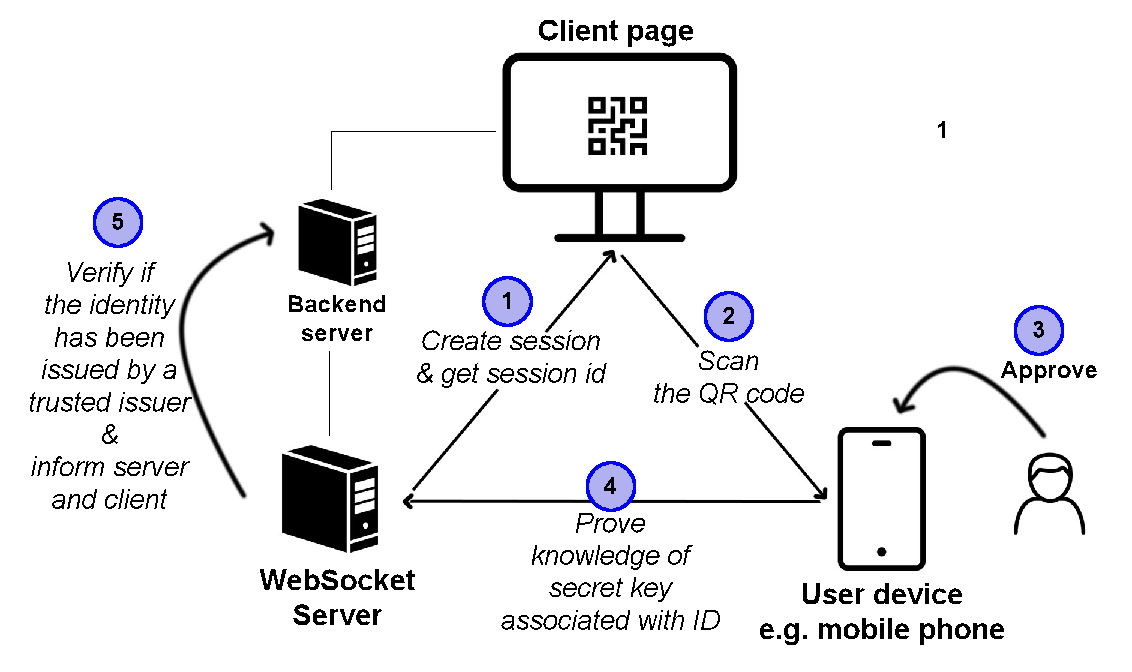
\includegraphics[scale=0.6]
    {figs/deeid/verifyanidentity.pdf}}
    \caption{Visualisation of how a traditional web page can authenticate a user's identity.\\\srcOwnFig}
    \label{fig:VerifyanIdentity}
\end{figure}

\subsection{Issuing an Identity}
We have described the system as dynamic and self-serving. This means that anyone and anything can issue an identity. This is done through the Fiat--Shamir scheme. Essentially, each issuer would have two large primes numbers that are kept secret, the product of these two are kept on the issuer's blockchain identity, i.e. smart-contract, so, when an identity holder claims to have been issued an identity, the verifier can check the existence of the product of the two large prime numbers within the issuers smart-contract or $\deeid_{\text{contract}}$.

Below we go through an example of how an identity is issued by any other participant on the network. The first box states the requirements and the necessary steps required before two participants can create identities for each other. In our implementation we created a flask (Python based) app that allowed a user to create an identity. Therefore, most organisations and current systems are able to do so without much development overhead.

In our implementation we created a Python function (described as $f$ throughout the chapter) that any developer can use to transform an identity string to a Fiat--Shamir public-key given the string, indices and $n$.


\noteBoxNormal{Example of Issuing an Identity}{%
    \begin{enumerate}
        \item \textbf{A: } Hand over the required identity bits, $I_1$ = \{Fullname, DoB, deeID, City of Birth\}
        \item \textbf{B: } Add a random string to $I_1$, and let that be $I$ hereafter.
        \item \textbf{B: } Verify the identity of $A$ (e.g. face to face by looking at passport etc.)
        \item \textbf{B: } If successful, create the credentials as follows:
        \begin{enumerate}
            \item Create the public-keys: $v_j = f(I,j)$ where $v_j$ is the public-key, $f$ is some pseudo-random function (\textit{Construction of such a function is explained in \cite{goldreich_how_1986}}) and $j$ are small random values; to create the public keys we pick $k$ distinct $j$ values for which $v_j$ is a quadratic residue $\mod n$, i.e. solution exists for $x^2 = v_j\mod(n)$
            \item Calculate the secret keys for $A$ by taking the smallest $s_j = \sqrt{v_j^{-1}} \bmod{n}$.
            \item So the set of $k$ public keys and associated $j$ values would give us two sets of values: $V = \{v_{j(1)}, v_{j(2)},\cdots,v_{j(k)}\}$ and $J = \{j_1, j_2,\cdots,j_k\}$
        \end{enumerate}
        \item Now $B$ can hand over $\{I, J, S, V\}$ to $A$. $V$ is technically not required because they can re-calculate it themselves if they have $I$ and $J$.
    \end{enumerate}
}
%\end{tcolorbox}

When an identity is issued, the state of the blockchain would not change; therefore there is no blockchain related costs associated with issuing new identities. The issuer would have the product of $p$ and $q$, $n$, within their smart-contract already, if not then the issuer would have to create a transaction and place $n$ within their \texttt{keys} array on the smart-contract, in this scenario there is an associated cost with this transaction.

\subsection{Verifying a Legal Identity}

By verifying a true identity, we mean that we are concerned with the actual real-life identity of the person. You can think of this as checking one's passport to get the real identity of the person we are concerned with. So, we have covered how you can issue an identity to someone, now we will go over how you can verify that identity. To give context, this would typically happen when one is applying for a credit card, insurance policy, or car finance online. Figure~\ref{fig:VerifyanIdentity} provides an overview of how we will proceed. We assume that the verifier (the backend and WebSocket servers) will have a set of trusted identity issuers \deeid addresses. Therefore, when they ask for an identity, they will ensure that the provided identity is provided by one of the trusted issuers. The actual authentication happens with the web server and the user's device (mobile phone); thus, for this to happen, the user has to first interact with the client, capture the required information, and then carry out the identification protocol with the WebSocket server. Upon the completion of the verification the server can update the client and carry out with the intended functions (e.g. registration and creating a session for the user).


%%%%%%%%%%%%%%%%%%%%%%%%%%%%%%%%%%%%%%%%%%%%%%%%%%%%%%%%%%%%%%%%55

\section{Evaluation}
\label{sec::chp6::evaluation}

This section evaluates the \deeid system using the framework proposed by Bonneau \etal\ in \textit{The Quest to Replace Passwords}~\cite{bonneau_quest_2012}. The framework assesses authentication schemes across three key dimensions: usability, deployability, and security. Figure~\ref{fig:deeIDComp} visually compares \deeid with other authentication schemes, and here, we systematically analyse how \deeid meets or falls short of each evaluation criterion, acknowledging its strengths and limitations.

\begin{figure*}[h]
    \centering
    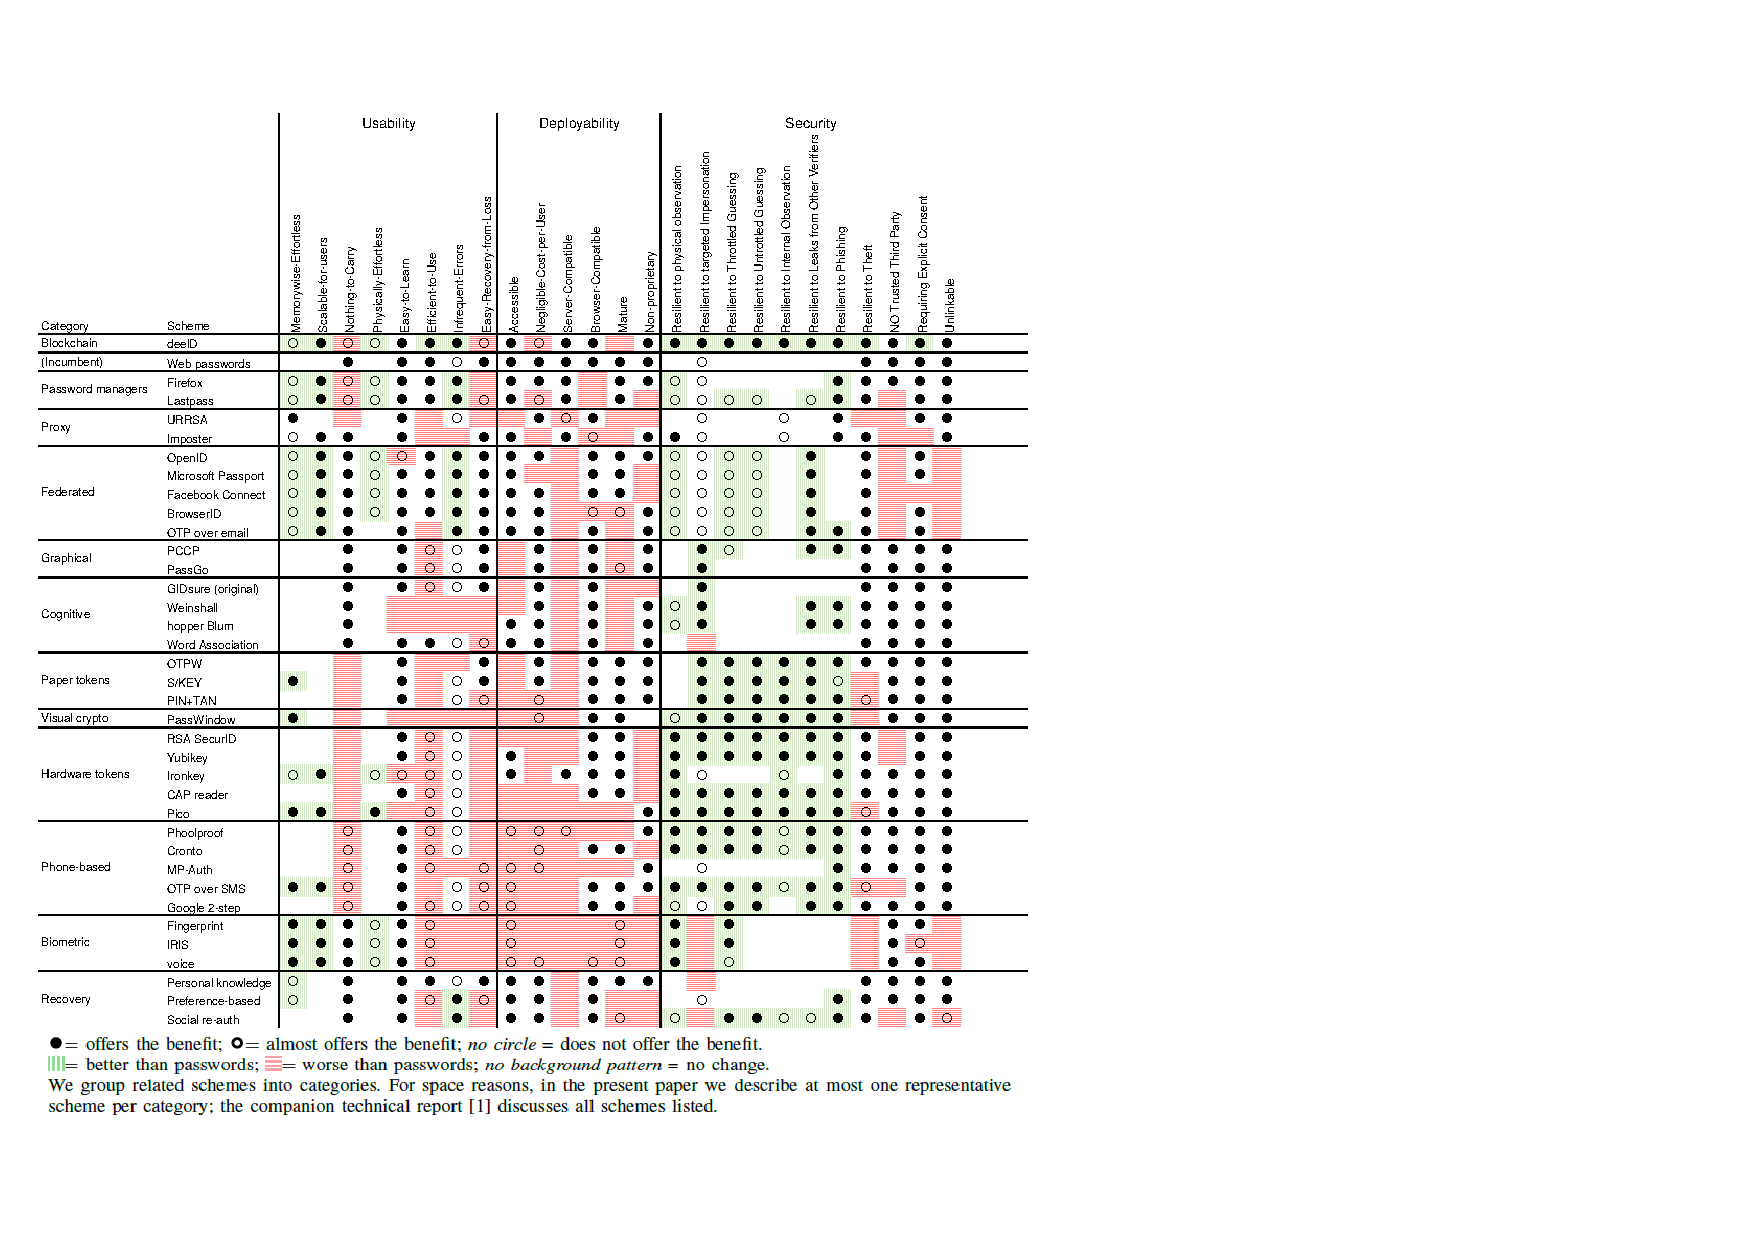
\includegraphics[trim={0 2cm 12cm 1cm},clip, scale=1]{figs/deeid/deeIDComparisonTable3.pdf}
    \caption{Visual evaluation of various schemes and our new blockchain-based scheme (\deeid).}
    \label{fig:deeIDComp}
\end{figure*}

\subsection{Usability Benefits}

\begin{enumerate}
    \item \textbf{Memorywise-Effortless}: There is no need for users to memorise passwords or other secrets; \deeid relies on a mobile phone device to store cryptographic secrets. This reduces cognitive load compared to traditional password systems. This benefit is similar to WebAuthn/Passkeys or password managers. However, the users may need to use a PIN to unlock their device.

    \item \textbf{Scalable-for-Users}: \deeid supports unlimited credentials and users can have multiple identities (issued from different organisations) without additional complexity. With the current system, there is a cost associated with transactions with the blockchain. Whilst this is a limitation of our method it is a technical challenge to overcome in future work. This benefit is similar to WebAuthn/Passkeys in regards to authentication.

    \item \textbf{Physically-Effortless}: Authentication and identification with \deeid requires scanning a QR code and pressing a button to confirm, a process that is physically straightforward and comparable to tapping a contactless card. There is a reliance on a mobile phone device and having it with you.

    \item \textbf{Easy-to-Learn}: \deeid is designed to be intuitive with minimal cognitive overhead. The actions and processes are familiar, such as scanning QR codes. The blockchain element is not easy to learn and most users are not required to learn or understand it; it can be abstracted away. Identity providers can provide onboarding and initial training if required.

    \item \textbf{Efficient-to-Use}: Authentication and identification is streamlined, requiring only a QR code scan and a single button press, making it faster than typing passwords or answering security questions. Compared to multi-factor authentication methods that involve multiple steps, \deeid offers a more efficient user experience. Network latency during blockchain queries may introduce minor delays.

    \item \textbf{Infrequent-Errors}: \deeid is reliable and deterministic. However, users would require their mobile phone device with them. Blockchain network issues might introduce errors or inconvenience.

    \item \textbf{Easy-Recovery-from-Loss}: This is a significant limitation of \deeid; there is no robust recovery mechanism. If a user loses their mobile device then they would not be able to recover their identity without backups. Users would need to get their identity re-issued from their providers.
\end{enumerate}


\subsection{Deployability Benefits}

\begin{enumerate}
    \item \textbf{Accessible}: The aim is to match or go beyond password's accessibility. Mobile phone devices are ubiquitous and most users have access to these devices with capability of securing cryptographic secrets on the hardware.  Accessibility is therefore high.

    \item \textbf{Negligible-Cost-per-User}: Blockchain transactions can incur charges, such as for issuing identities or updating contracts. The user requires a mobile phone which can be costly. Beyond these costs, all identity verifications and authentications have no costs associated with them.

    \item \textbf{Server-Compatible}: Compatibility with existing tech stacks were a key requirement in the design stage. \deeid requires no specialised server-side infrastructure unless a blockchain needs to be installed. Most organisations would be able to implement the password-less authentication feature easily. 

    \item \textbf{Browser-Compatible}: Do users need client change or additional software? It would be quasi-compatible if it reliance on common plugins like Flash. \deeid is a compatible with most modern browsers.

    \item \textbf{Mature-Technology}: \deeid uses mature technologies as the building block, however in itself it is not a mature technology or widely adopted. Maturity and adoption of this \deeid requires recognition amongst large technology organisations that control distribution.

    \item \textbf{Non-Proprietary}: This is where anyone can implement or use the scheme without royalties (not protected by patent or trade secrets). \deeid is designed and developed on open technologies such as Ethereum, the Fiat--Shamir cryptosystem, and other widely available client-server technologies.
\end{enumerate}


\subsection{Security Benefits}

\begin{enumerate}
    \item \textbf{Resilient-to-Physical-Observation}: No secrets are displayed or entered during authentication. The QR code displayed can be timed or randomised at a rapid rate. All operations occur on the user's device. The zero-knowledge properties of the protocols used means no secret information is revealed.

    \item \textbf{Resilient-to-Targeted-Impersonation}: Skilled or well-resourced malicious actors would not be able to impersonate the user unless the user's mobile phone device is stolen and the attacker can access it. \deeid is resilient against phishing attacks and other social engineering attacks.

    \item \textbf{Resilient-to-Throttled-Guessing}: Secrets are not stored on centralised servers, they are held on the user's device. It is computationally infeasible to attempt to guess the users's Fiat--Shamir secrets, especially with large key sizes.

    \item \textbf{Resilient-to-Unthrottled-Guessing}: Similar to throttled guessing, this is also unfeasible due to the nature of the cryptosystems used and lack of credential centralisation.

    \item \textbf{Resilient-to-Internal-Observation}: If a user interacts with a service on the client then they are secure against attacks, such as the Man-in-the-Browser malware. The users do not interact with the cryptographic secrets on the mobile phone, if stored on the secure enclaves then they are unobservable.

    \item \textbf{Resilient-to-Phishing}: The zero-knowledge nature of \deeid’s authentication ensures that no secret information is shared with verifiers. The operations on the mobile phone, where a service is authenticated, ensures that the user is unlikely to be phisehd.

    \item \textbf{Resilient-to-Theft}: The system is resilient-to-theft if a physical object cannot be used for authentication or identification by another user. It would be quasi-resilient-to-theft if protected by a PIN without rate control. \deeid is quasi-resilient-to-theft as the mobile phone device is likely to have a PIN or biometric. Future work can focus on making this aspect more secure.

    \item \textbf{No-Trusted-Third-Party}: \deeid uses a trusted third party to create an identity on the blockchain. Beyond this initial setup, \deeid does not use any other trusted third parties.

    \item \textbf{Requiring-Explicit-Consent}: Authentication and identification requires an explicit action from the user, such as scanning a QR code or pressing a button. This ensures authorised access and accidental or drive-by identification.

    \item \textbf{Unlinkable}: If the user is carrying out identification, then they are linkable due to their unique identity. However, if they carry out authentication (without the use of the blockchain), then it will be unlinkable, unless the services track the users by other means.
\end{enumerate}





\section{Discussion}
\label{sec::chp6::discussion}

One of the primary strengths of \deeid is in its extension of the Fiat--Shamir identification protocol to accommodate multiple identity issuers. Unlike traditional systems that rely on a single trusted authority or on centralised certificate authorities, \deeid's use of blockchain as a DPKI enables a dynamic trust network where any organisation—be it a bank, government, or university—can issue verifiable credentials. This decentralisation eliminates single points of failure and reduces the risk of systemic compromise, as demonstrated by real-world incidents such as the SEC Twitter/X account hack via SIM swapping \cite{kan_hijack_2024} or the deepfake-enabled US\$25 million fraud \cite{milmo_uk_2024}. By replacing shared secrets with zero-knowledge proofs, \deeid ensures that no reusable information is exposed during verification, significantly reducing the attack surface for impersonation and replay attacks.

%The system's compatibility with existing web technologies is another critical advantage. By utilizing QR codes, WebSocket communication, and standard JavaScript or Python libraries, \deeid integrates seamlessly with current web infrastructure without requiring browser modifications or proprietary software. This deployability makes it practical for organizations to adopt \deeid without overhauling their existing systems, addressing a common barrier to the adoption of advanced authentication schemes \cite{bonneau_quest_2012}. Furthermore, the support for multiple authentication methods—ranging from explicit blockchain-based links to anonymous public-key generation—offers flexibility to cater to diverse use cases, from high-security scenarios requiring strong identification to privacy-focused applications needing unlinkable authentication.

\deeid has taken a privacy-by-design approach. By employing zero-knowledge proofs, the system ensures that verifiers receive only the information necessary for authentication/identification, protecting users from oversharing sensitive data. This aligns with growing regulatory demands for data minimisation, such as those outlined in the GDPR and similar frameworks. Additionally, the ability to support multiple devices and keys enhances usability, allowing users to manage their identities across various contexts without being locked into a single vendor or ecosystem, unlike federated identity systems.

%Human identification is an integral part of the security of the digital ecosystem. Though it is a missing element at the moment which is leading to account breaches, identity theft, and much more. In this chapter, we introduced the Fiat--Shamir scheme and have generalised it so that it could work on a larger scale with \textit{multiple} identity issuers. Our solution has been to use the blockchain as a decentralised PKI. Blockchain-based PKIs have shown promise in research and applications. Emergence of blockchain-based PKIs have come about mainly due to the weak-link security problem with respect to certificate authorities and the X.509 standard~\cite{noauthor_x.509_nodate} (other main PKI standard is OpenPGP~\cite{shaw_openpgp_nodate}). Consequently, this has led to new approaches such as the Google Certificate Transparency project~\cite{noauthor_certificatetr_nodate}. Blockchain PKI models such as~\cite{konoplev_blockchain_2018} attempt to overcome the weaknesses of current PKI standards.

% Essentially we have a p2p network and we have to represent the human identities on this network. How should the identity be represented? and what mechanisms are required to interact with the identity? Going back to our four rules: a) Capture: each identity must have a unique representation on the network. Each \deeid\ contract has a unique address. b) Recording: It must be machine and human readable. The \deeid\ contract address is unique and machine-readable. The user can also prove their identity and give their human readable names to the challenger. c) Security: can we protect from impersonation and other attacks? Best current method is using public-key cryptography and \textit{what we posses} rather than \textit{what we know} or \textit{what we are}. d) Verification: Using the mobile phone device and the Fiat--Shamir scheme we can verify identities easily.

%Similar to uPort we have represented the identity by a smart-contract which is uniquely identified in the network. Therefore, each identity has an interactive code on the network (managed by the identity holder themselves). So, here, identity is no longer a piece of string such as your full name, but a totally unique digital representation on a network. The benefit of this is that it is a single-source of truth that everyone can use and agree upon. So, your bank, hospital and school can all use the same identity. Using the same identity and authentication scheme can provide data sharing which in itself has huge benefits. We believe merging the Fiat--Shamir scheme with the existing blockchain identity methods is a novel method for an identification system.

%The benefit of using the Fiat--Shamir scheme over simply signing an identity string is the privacy and security it provides. Moreover it saves transactions and space on the network. However, it is still important to keep our 'full names', the basic string identity, because we humans still need to communicate with one another and be able to identify each other. Which is not possible if we are identified by a 512bit unique identity string. There have been studies such as \cite{bonneau_towards_2014}, \textit{'Towards reliable storage of 56-bit secrets in human memory'}, where the authors tried to see if we humans can remember long bits of string. The conclusion was that humans are able to learn cryptographic secrets (56-bit in this case), though it requires significant learning periods and other limitations such as recalling times.

%The issue of how do we trust the identity issuer falls upon the verifier. At the moment it is conceived to be a simple linear trace back of identities until the final link must somehow be verified. In our implementation we have a simple link to an official website or regulatory-body portal. However, there is considerable work to be done in improving this, e.g. one can quantify trust and provide recommendation to the verifier whether they are trust-worthy. A reputation-based network can provide some metric for verifiers to work from. However, one must consider the ethical implications of quantifying reputation, especially when we are considering real identities.

%\deeid predates Passkeys but offers similar advantages to it and WebAuthn when it comes to password-less authentication. Traditional authentication systems expose users to compromise when websites, third-party libraries, browsers, or operating systems contain vulnerabilities, as demonstrated by the 2018 British Airways breach where attackers compromised website scripts to steal customer data during entry, including CVV numbers that organizations typically never store~\cite{noauthor_british_2019, bishop_this_nodate}. In contrast, \deeid eliminates these input-capture vulnerabilities by using QR code scanning to initiate encrypted WebSocket connections that bypass browser-based data entry entirely, preventing scrapers and compromised web components from intercepting authentication credentials. The system employs public-key cryptography and digital signature schemes rather than passwords, providing four distinct authentication methods through public keys stored on users' identity smart contracts. This architecture enables users to manage their own security posture by adding or removing cryptographic keys as needed, offering both enhanced security and user autonomy compared to centralised password-based systems that remain vulnerable to website-level compromises.

When compared to existing authentication systems like WebAuthn and Passkeys, \deeid stands out for its focus on identification rather than solely authentication. While WebAuthn effectively addresses password-less authentication through public-key cryptography, it does not inherently support the complex, multi-issuer identity verification scenarios that \deeid targets. For instance, WebAuthn is primarily designed for single-site authentication, whereas \deeid enables cross-organisational identity verification through its blockchain-based trust network. This makes \deeid particularly suited for applications requiring robust identity verification, such as financial services, healthcare, or government services, where multiple trusted issuers are involved.

Traditional public key infrastructures (PKIs) rely on centralised certificate authorities, which introduce vulnerabilities such as single points of failure and potential coercion. In contrast, \deeid's blockchain-based DPKI distributes trust across a decentralised network, reducing reliance on any single entity. Compared to other blockchain-based identity systems like Namecoin \cite{noauthor_namecoin_nodate} or Certcoin \cite{fromknecht_certcoin_2014}, \deeid's integration of the Fiat--Shamir protocol with a multi-issuer framework provides a more flexible and scalable solution for real-world identity management. Additionally, \deeid's emphasis on zero-knowledge proofs distinguishes it from systems like Blockstack \cite{noauthor_blockstack_nodate}, which may not prioritise privacy to the same extent.


% In our evaluation we followed the framework described in \cite{bonneau_quest_2012} to do a comparative analysis of \deeid with existing authentication schemes. Schemes such as: passwords, password managers, federated systems, hardware, mobile phone based systems, biometrics and more. The \deeid protocol uses cryptographic keys that are unpractical for humans to read, copy and transfer themselves without the help of a machine. Moreover, the computation required for these keys is impossible for humans to do. Thus, the use of a machine such as a mobile phone is required. Consequently, our protocol blurs the lines between hardware tokens, phone-based systems, federated and password management systems as shown in Figure~\ref{fig:deeIDArchitecture}.

% It should be noted that the framework in Figure~\ref{fig:deeIDArchitecture} is designed for human practicality, incorporating factors such as ``nothing to carry'', ``physical-effortlessness'' and ``memory-wise-effortless''. Therefore, the protocols are highly human-centric at present. Nevertheless, as we progress into the domains of AI and IoT, we can improve upon these protocols and frameworks to accommodate other non-human entities as well. Whilst no other system can surpass passwords that are easily stored and retrieved in our brains, as the number of passwords to remember increases, we encounter difficulties. Thus, the benefits of alternative schemes, such as password managers, become more apparent.


Preventing SIM swap attack is another use case of \deeid. SIM swap attack is where an attacker uses social-engineering (operator error and weakness) to convince the user's mobile carrier to swap the SIM to the attacker's SIM. The consequence of this is that the attacker can hijack accounts that use two-factor authentication (2FA). Notable hacks include the hijacking of celebrity Instagram accounts~\cite{bell_instagram_nodate} and individuals losing millions of pounds of cryptocurrency as their exchange accounts were linked to their mobile phone number using 2FA. This is a growing threat that is leading to more organised crime~\cite{franceschi-bicchierai_sim_2018}. Preventive techniques include using a PIN or better 2FA~\cite{wire_protect_swimswap}. However, these are patchy and preventive measures; a standardised solution through the use of decentralised identity like that of \deeid\ across mobile network carriers would be a better solution. Explicitly linking the user's \deeid\ to their SIM and having a hardware linked crypto keys - meaning that it is physical and malicious attackers cannot carry out their attack without access to the physical elements. When the SIM is linked to the user's \deeid\ (do this when the user acquires the SIM), the attacker would have to identity themselves which is far more difficult that knowing the user's name, address and date of birth.

Mitigating identity theft presents a compelling use case for \deeid, as current credit verification systems enable attackers to obtain credit cards using only a victim's name, address, and date of birth. This vulnerability stems from credit agencies operating on a ``pull'' model, where third parties can access credit reports by providing basic personal information, rather than a ``push'' model requiring explicit authorization from the identity owner. Under a \deeid-based framework, credit agencies such as Experian~\cite{noauthor_experian_nodate}, Equifax~\cite{noauthor_equifax_nodate}, and TransUnion~\cite{noauthor_transunion_nodate} would link customer data to individual \deeid credentials, transforming credit inquiries into authorization requests that require explicit consent from the identity owner before releasing information. While the economic implications of such systemic changes present significant implementation challenges, establishing this intermediary authentication layer would provide technically sophisticated users with substantially greater control over their personal credit information and enhanced protection against unauthorized access.

\section{Limitations}
\label{sec::chp6::limitations}

We have not completely eliminated trusted third parties (identity issuers) from our system. Can we ever fully remove them? We believe not. However, our system requires trusted third parties only when identities are first created. Future work could consider reputation systems for the identity issuers.

The identity issuers are currently unable to revoke an identity. If an identity is compromised or the user has lost their secrets related to that identity then the identity issuer should be able to revoke that identity so no other party can use it.

There is no feature to \textit{recover an identity}. If a user loses their mobile phone device with their secrets then they won't be able to get prove their identities any more unless they have backups. Currently, there is no equivalent of ``Forgot my password''.

Mobile device dependence creates usability barriers and single points of failure. We do not run a blockchain node on the device and would therefore need to have a trusted node to communicate with. Future work could focus on dedicated hardware to carry out the main \deeid functions.

When an identity is proved, the user reveals all \textit{identity bits}. This limitation means that the user is oversharing information and leads to privacy concerns. Future work could consider selective disclosure of identity bits (such as date of birth or just birth year if they only need to prove their age).

\noteBox{Future Work: Selective Disclosure}{%
Treating services as adversarial dictates that we must minimise shared information bits. While Fiat--Shamir zero-knowledge cryptosystems ensure that secrets themselves are not disclosed, they still require revealing various attributes of our identity. However, in real-world scenarios, a prover often needs to disclose only some attributes rather than all. For example, someone proving that they are German does not need to reveal other identity attributes. This is where \textit{Selective Disclosure} of identity attributes becomes crucial. We can combine the Fiat--Shamir~\cite{fiat_how_1987} cryptosystem with a Merkle~tree~\cite{merkle1987digital} construction to selectively reveal certain attributes while keeping others hidden.
}

Well-resourced malicious actors and nation-states threaten blockchain networks. These attackers can destabilise networks or disable them entirely by launching coordinated attacks such as 51\% attacks, eclipse attacks, or distributed denial-of-service campaigns.

We developed our implementation on Ethereum, which relies on a Proof-of-Work consensus mechanism. However, Proof-of-Work creates two significant problems: it consumes an excessive amount of energy and requires us to trust miners whom we cannot verify. For identity management networks, we need better alternatives. Proof-of-Stake offers one solution, while Proof-of-Reputation \cite{zhuang_proofofwork_2019} provides a more experimental approach. Both schemes would serve identity management networks more effectively than Proof-of-Work, as they address its core limitations while supporting the specific requirements of identity systems.

\section{Summary}
\label{sec::deeid::summary}

In this chapter we have broken down the idea of identity, its representation and definition and explored how one can one uniquely identify themselves. We have compared our blockchain-based identity system with existing systems and typical password systems. We have argued that \deeid provides better security than federated, mobile phone-based, and hardware-based systems which in turn provide better security than passwords. Deployability is where most schemes fall back on compared to passwords. However, this is something that cannot be beaten due to 'knowing something' is more deployable than all other systems. Given that our system can inherently be a password manager too, it therefore strikes a better balance between the three major comparison factors of usability, deployability and security.

\deeid can also be built on top of other blockchain technologies. Our novel contribution is improving upon identity representation through smart-contracts, allowing the blockchain as a cryptographic key management and a trusted-source of identities and providing a mechanism for people on the network to provide identities to one another. This was achieved by allowing the Fiat--Shamir scheme to have multiple identity issuers through the blockchain. This is most useful in the real world where multiple organisations can issue identities to the same individual.

Future work can be separated into four different pillars, (1) General algorithm optimisation of the Fiat--Shamir cryptosystem. (2) We believe that an identity system such as the one proposed in this chapter could become an integral part of future blockchain systems that utilise Proof-of-Authority consensus schemes. A \deeid based Proof-of-Authority that is Byzantine Fault Tolerant with some quantifiable method for reputation to manage the network, (3) We have skewed our approach towards human identity, the definition can be debated, however one can extend the scheme to go beyond humans and make it a universal identity system for entities that include IoT devices, animals, fictional entities, and even cyborgs with vision of a decentralised galactic identity network. (4) Lastly, our design has been blockchain implementation agnostic, therefore one can think about interoperability of the scheme and how identities across networks can interact with one another.
